\begin{center}
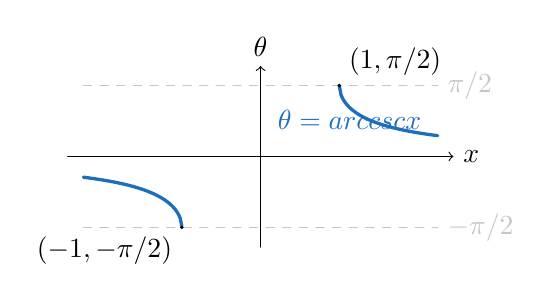
\begin{tikzpicture}[scale=1.0, line cap=round, line join=round]
  \definecolor{trigblue}{RGB}{30,110,190}
  \draw[->] (-2.45,0)--(2.45,0) node[right] {$x$};
  \draw[->] (0,-1.15)--(0,1.15) node[above] {$\theta$};
  \draw[gray!45,dashed] (-2.25,0.9)--(2.25,0.9) node[right] {$\pi/2$};
  \draw[gray!45,dashed] (-2.25,-0.9)--(2.25,-0.9) node[right] {$-\pi/2$};
  \draw[very thick,trigblue,domain=1:2.25,samples=60]
    plot ({\x},{0.9*asin(1/\x)/90});
  \draw[very thick,trigblue,domain=-2.25:-1,samples=60]
    plot ({\x},{0.9*asin(1/\x)/90});
  \fill (1,0.9) circle (0.025) node[above right] {$(1,\pi/2)$};
  \fill (-1,-0.9) circle (0.025) node[below left] {$(-1,-\pi/2)$};
  \node[trigblue] at (1.13,0.47) {$\theta=\operatorname{arccsc} x$};
\end{tikzpicture}
\end{center}
